\section*{Лекция 12 (05.05.2022)}

\subsection{Непрерывность неявного отображения}

\begin{namedlemma}{Обратимость линейного отображения, близкого к тождественному}
    $Y$ -- полное нормированное пространство. $U \in L(Y, Y)$, $\norm{U} < 1$, $I$ -- тождественное. Тогда $\exists (I \pm U)^{-1} \in L(Y, Y)$.
\end{namedlemma}
\begin{proof}
    \item[1 способ.] Хотим доказать, что $\forall u \in Y \exists! y \in Y \colon (I - U)u = u$ \\
    $y - Uy = u \Leftrightarrow y = u + Uy$\\
    $g_u \colon Y \to Y$, $g_u(y) = u + Uy$, хотим показать, что $g_u$ -- сжимающее.\\
    $\norm{g_u(y_1) - g_u(y_2)} = \norm{Uy_1 - Uy_2} \leqslant \norm{U} \cdot \norm{y_1 - y_2} \Rightarrow \exists! y_0 \colon y_0 = u + Uy_0$. \\
    Отсюда, $I - U$ биекция, аналогично $I + U$.

    Теперь проверим, что $(I - U)^{-1}$ -- непрерывное отображение. Сделаем это по определению, пусть $u_n \to u_0$, по $u$ однозначно строится $y = u + Uy$, пусть это $y_n$ и $y_0$ соответственно. Хотим показать, что $y_n \to y_0$. \\
    $\left\{\begin{aligned}
    (I - U) y_n = u_n \\
    (I - U) y_0 = u_0
    \end{aligned}\right. \Rightarrow (I - U_n) (y_n - y_0) = u_n - u_0 \Rightarrow y_n - y_0 = u_n - u_0 + U (y_n - y_0) \Rightarrow \norm{y_n - y_0} \leqslant \norm{u_n - u_0} + \norm{U} \norm{y_n - y_0}$\\
    $0 \leqslant (1 - \norm{U}) \norm{y_n - y_0} \leqslant \norm{u_n - u_0} \to 0 \Rightarrow y_n \to y_0$.
    \item[2 способ.] Докажем, что $(I - U)^{-1} = I + U + U^2 + \ldots$ -- сходится абсолютно, то есть сходится ряд $\norm{I} + \norm{U} + \norm{U^2} + \ldots$.\\
    $\norm{U^n} \leqslant \norm{U}^n \Rightarrow \sum\limits_{i = 0}^{\infty} \norm{U^i} \leqslant \sum\limits_{i = 0}^{\infty} \norm{U}^i = \dfrac{1}{1 - \norm{U}}$.\\
    $L(Y, Y) -$ полное, так как $Y -$ полное, поэтому по критерию Коши из абсолютной сходимости следует обычная.\\
    $S_n = I + U + \ldots + U^n \stackrel{n \to \infty}{\longrightarrow} S \in L(Y, Y)$.\\
    $\underset{\substack{\downarrow \\ (I - U)S}}{(I - U)S_n}= \underset{\substack{\downarrow \\ S(I - U)}}{S_n(I - U)} = I - U^{n + 1} \stackrel{n \to \infty}{\longrightarrow} I$
\end{proof}

\begin{lemma}
    $U \in L(Y, Z)$, $\exists U^{-1} \in L(Z, Y) \quad \forall V \in L(Y, Z) \quad \norm{V} < \dfrac1{\norm{U^{-1}}} \Rightarrow \exists (U \pm V)^{-1} \in L(Z, Y)$, $Y$ - полное.
\end{lemma}
\begin{proof}
    $(I + VU^{-1})U = U + V = U(I + U^{-1}V)$.\\
    $\norm{U^{-1}V} < 1 \stackrel{\text{л. 1}}{\Rightarrow} \exists (I + U^{-1}V)^{-1} \Rightarrow$
    $(U(I + U^{-1}V))^{-1} = (I + U^{-1}V)^{-1}U^{-1}$.
\end{proof}

\begin{theorem}
    Если в условии теоремы \link{о неявном отображении} потребовать непрерывность $G$ и $\partial y G$ не только в точке $(x_0, y_0)$, но и в целой окрестности, то постренная $f$ будет непрерывна в некоторой окрестности $x_0$.
\end{theorem}
\begin{proof}
    Если $(x_1, y_1)$ близка к $(x_0, y_0)$, тогда $V = \partial y G(x_1, y_1) - \partial y G(x_0, y_0) \stackrel{(x_1, y_1) \to (x_0, y_0)}{\longrightarrow} 0$, отсюда по лемме $\exists (\partial y G(x_1, y_1))^{-1} \in L(Z, Y) \Rightarrow (x_1, y_1)$ удовлетворяет условиям теоремы о неявном отображении и $f$ непрерывна в точке $x_1$.
\end{proof}

\begin{theorem}
    Если в дополнение к условиям теоремы \link{о неявном отображении} выполнено условие дифф $G$ в точке $(x_0, y_0)$, то $f$ дифференцируема в точке $x_0$, и $d f(x_0) = - (\partial y G(x_0, y_0))^{-1} \partial x G(x_0, y_0)$
\end{theorem}
\begin{proof}
    $G(x,y) = G(x_0, y_0) + \partial x G(x_0, y_0) (x - x_0) + \partial y G(x_0, y_0) (y - y_0) + o (\norm{x - x_0} + \norm{y - y_0})$.\\
    $\exists V_0, U_0 \colon G(x, y) = 0 \quad \forall (x, y) \in U \times V \Leftrightarrow y = f(x) \quad \forall x \in U \Rightarrow \\ 0 = G(x, f(x)) = \partial x G(x_0, y_0) (x - x_0) + \partial y G(x_0, y_0) (f(x) - f(x_0)) + o(\ldots) \Rightarrow$
    \begin{equation}
        \label{*}
        f(x) - f(x_0) = - (\partial y G(x_0, y_0))^{-1} \partial x G(x_0, y_0) (x - x_0) + (\partial y G(x_0, y_0))^{-1}o(\ldots)
    \end{equation}
    Хотим $\norm{y - y_0} \leqslant \norm{x - x_0} \Rightarrow o(\norm{x - x_0}) = o(\norm{x - x_0} + \norm{y - y_0})$\\
    $\ref{*} \Rightarrow \norm{y - y_0} \leqslant C_1 \norm{x - x_0} + C_2\epsilon (\norm{x - x_0} + \norm{y - y_0}) \ \forall \epsilon > 0$, где\\
    $\begin{aligned}
    C_1 &= \norm{(\partial y G(x_0, y_0))^{-1})} \cdot \norm{\partial x G(x_0, y_0)} \\
    C_2 &= \norm{(\partial y G(x_0, y_0))^{-1})}
    \end{aligned}$.\\
    Тогда подобрав подходящий $\left(< \dfrac{1}{C_2}\right)$ $\epsilon$, получим, что $\norm{y - y_0} \leqslant C \norm{x - x_0}$, из чего последует дифференцируемость $f$ в точке $x_0$.
\end{proof}

\follow Если хочется, чтобы $f$ была $k$ раз дифференцируема, достаточно потребовать, чтобы $G$ была $k$ раз дифференцируема.

\subsection{Теорема об обратном отображении}
\begin{theorem}[об обратном отображении]
    $F \colon Y \to X \quad F(y_0) = x_0 \quad F$ дифференцируема в окрестности точки $y_0$, $\exists (d F(y_0))^{-1} \in L(X, Y) \Rightarrow \exists U, V$ -- окрестности $x_0, y_0 \colon F \colon V \to U -$ биекция, т. е. $\exists F^{-1} = f$, а так же $(dF^{-1})(x_0) = (d F(y_0))^{-1}$
\end{theorem}
\begin{proof}
    $G \colon X \times Y \to X$ $G(x, y) = x - F(y)$, заметим что для такого $G$ выполнены условия теоремы \link{о неявном отображении}: $\partial y G(x_0, y_0) = -d F(y_0)$, $G(x_0, y_0) = 0$, так же очевидно, что $G$ и $\partial y G$ в точке $(x_0, y_0)$.\\
    Тогда $\exists U$ -- окрестность $x_0$, $V$ -- окрестность $y_0 \colon x = F(y) \Leftrightarrow G(x, y) = 0 \quad (x, y) \in U \times V \Leftrightarrow y = f(x) \quad x \in U$.\\
    Заметим, что мы еще не получили биекцию, так как из равносильности следует только инъективность $f$, так как она не насыщает все точки образа. С этим можно побороться, если взять вместо $V := f(U)$, но тогда нужно доказать, что $y_0$ было внутренней для $f(U)$.\\
    Тогда давайте посмотрим на дифференциал $f$, $df(x_0) = -(\partial y G(x_0, y_0))^{-1} \partial x G(x_0, y_0) = (d F(y_0))^{-1} \Rightarrow \exists (d f(x_0))^{-1} = d F(x_0) \in L(Y, X)$.\\
    Отсюда получим, что можно применить рассуждения выше для функции $f$ и получить окрестности $U_0, V_0$, тогда итоговые будут равны $U \cap U_0$ и $V \cap V_0$ и в них $f$ будет биекцией.
\end{proof}

\subsection{Условные экстремумы}

\underline{Постановка} Есть поверхность, хотим минимизировать / максимизировать $f$ на поверхности

\tikzset{every picture/.style={line width=0.75pt}} %set default line width to 0.75pt

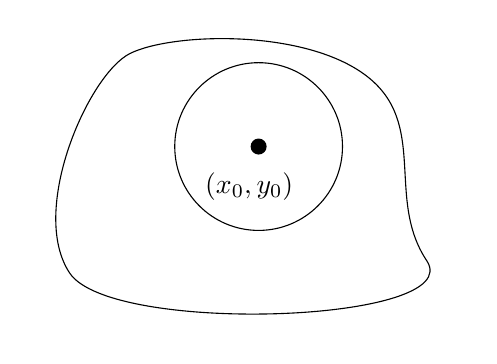
\begin{tikzpicture}[x=0.75pt,y=0.75pt,yscale=-1,xscale=1]
%uncomment if require: \path (0,300); %set diagram left start at 0, and has height of 300

%Shape: Polygon Curved [id:ds7711242767337856]
\draw   (170,74) .. controls (190,64) and (254,61.81) .. (284,84.81) .. controls (314,107.81) and (293,143.81) .. (313,173.81) .. controls (333,203.81) and (161,209.81) .. (141,179.81) .. controls (121,149.81) and (150,84) .. (170,74) -- cycle ;
%Straight Lines [id:da45347310606748215]
\draw    (227,130.81) ;
%Straight Lines [id:da7295066472606988]
\draw    (232,118.81) ;
\draw [shift={(232,118.81)}, rotate = 0] [color={rgb, 255:red, 0; green, 0; blue, 0 }  ][fill={rgb, 255:red, 0; green, 0; blue, 0 }  ][line width=0.75]      (0, 0) circle [x radius= 3.35, y radius= 3.35]   ;
%Shape: Circle [id:dp7806868550594233]
\draw   (191.59,118.81) .. controls (191.59,96.5) and (209.68,78.41) .. (232,78.41) .. controls (254.32,78.41) and (272.41,96.5) .. (272.41,118.81) .. controls (272.41,141.13) and (254.32,159.22) .. (232,159.22) .. controls (209.68,159.22) and (191.59,141.13) .. (191.59,118.81) -- cycle ;

% Text Node
\draw (205,130.21) node [anchor=north west][inner sep=0.75pt]    {$( x_{0} ,y_{0})$};


\end{tikzpicture}

$X, Z$ -- метрические пространства, $\Phi \colon X \to Z$, $M = \{x \colon \Phi(x) = 0\}$ -- поверхность уровня $\Phi$, $f \colon W \subset X \to \R$.

\begin{definition}
    $x_0$ -- точка условного локального минимума $f$ при условии $\Phi = 0$, если $\Phi(x_0) = 0$ и $\exists \widetilde{W}$ -- окрестность $x_0 \colon \forall x \in \widetilde{W} \cap M$ $f(x) \geqslant f(x_0)$.
\end{definition}

$\Phi - \text{дифференцируема} \colon \R^{m + n} \to \R^n$ $\Phi(x_1, \ldots, x_{m + n}) = 0 \Leftrightarrow \left\{\begin{aligned}
\Phi_1(x_1, \ldots, x_m,& \ldots, x_{m + n}) = 0 \\
&\vdots \\
\Phi_n(x_1, \ldots, x_m,& \ldots, x_{m + n}) = 0
\end{aligned}\right.$\\
Рассмотрим матрицу Якоби этого отображения,
$\begin{pmatrix}
\dfrac{\partial \Phi_1}{\partial x_1} & \cdots & \dfrac{\partial \Phi_1}{\partial x_{n + m}} \\
\vdots & \ddots & \vdots \\
\dfrac{\partial \Phi_n}{\partial x_1} & \cdots & \dfrac{\partial \Phi_1}{\partial x_{n + m}}
\end{pmatrix}$\\
Если ранг этой матрцы максимален и равен $n$, тогда можно выбрать $n$ линейно независимых столбцов, переставить их в конец и обозначить $y_1, \ldots, y_n$. Тогда мы получим $\Phi_j(x_1, \ldots, x_m, y_1, \ldots, y_m)$, $\partial y \Phi(x, y) = \left(\dfrac{\partial \Phi_j}{\partial y_k}\right)$ -- обратимая, поэтому по теореме о неявном отображении, $\{(x, y) \mid \Phi(x, y) = 0\}$ -- график отображения $y = \varphi(x)$.\\
И задача сводится к тому, чтобы локально минимизировать функцию $f(x_1, \ldots, x_m, y_1, \ldots, y_m) = f(x_1, \ldots, x_m, \varphi(x_1, \ldots, x_m)) = \widetilde{f}(x_1, \ldots, x_m)$.\\
Искать условный экстремум $f$ при условии $\Phi = 0 \Leftrightarrow$ искать экстремум функции $\widetilde{f}$.
